% !TEX root = ../main.tex
\chapter{Empirical Methodology and Results}

\section{Estimation Strategy}

The primary challenge in estimating the impact of the Hurricane Ian shock on remittance inflows to Mexican municipalities lies in the sorting of migrants. Municipalities with higher exposure to Florida may differ systematically from those with networks concentrated in other U.S. states. Therefore, a standard cross-sectional analysis comparing municipalities with different levels of exposure to Florida would likely lead to biased estimates due to confounding factors correlated with both the treatment (i.e. exposure to Florida) and the outcome (i.e. remittance inflows). This classic omitted variable bias problem makes a causal interpretation of cross-sectional estimates impossible \parencite{wooldridge2010}. To overcome this challenge, we leverage the temporal variation in remittance inflows by employing a continuous Difference-in-Differences (DiD) event-study design \parencite{callaway2024}, where our treatment is the pre-shock exposure to Florida, measured by $w_{m,\text{FL}}$. 

\section{Event-Study Specification}

We use the following Poisson Pseudo Maximum Likelihood (PPML) event-study specification to analyze the impact of the Hurricane Ian shock on remittance inflows to Mexican municipalities:
\begin{equation} \label{eq:ppml-event-study}
\mathbb{E}[R_{mt} \mid \mathbf{X}_{mt}] = \exp \left( \alpha_m + \gamma_{s(m),t} + \sum_{k \neq -1} \beta_k \cdot \left( w_{m,\text{FL}} \cdot \mathbbm{1}\{t - T_0 = k\} \right) \right)
\end{equation}
This methodology is motivated by \cite{silva_tenreyro_2006}, who show that the PPML estimator remains consistent in the presence of heteroskedasticity and excess zeros, which are common features of remittance data at the municipality level. The event-study specification allows us to estimate the dynamic treatment effects of the shock over time. We include municipality fixed effects ($\alpha_m$) to control for all time-invariant, unobserved municipal characteristics that might otherwise introduce omitted variable bias. Additionally, we incorporate state-by-time fixed effects ($\gamma_{s(m),t}$), where $s(m)$ denotes the specific Mexican state to which municipality $m$ belongs. These fixed effects account for both macroeconomic shocks common to all regions and time-varying unobservables at the state level. The interaction term $w_{m,\text{FL}} \cdot \mathbbm{1}\{t - T_0 = k \}$ captures the differential effect of the shock on Mexican municipalities based on their varying degrees of baseline exposure to Florida, where $w_{m,\text{FL}}$ is a measure of pre-shock exposure to Florida and $\mathbbm{1}\{t - T_0 = k \}$ is an indicator for each time period relative to the shock. The coefficients $\beta_k$ thus represent the change in remittance inflows for a one-percent increase in Florida exposure at each time period $k$ relative to the shock. Errors are clustered at the municipality level to account for potential correlation within municipalities over time.

\section{Robustness Checks}

The consistency of the PPML estimator relies only on the assumption that the conditional mean is correctly specified \parencite{silva_tenreyro_2006}. Unlike the log-linear model, it requires no assumption on the conditional variance, so heteroskedasticity and overdispersion do not threaten consistency; they affect only efficiency and inference, which we handle through standard errors clustered by municipality. This narrows the robustness exercise to two questions: whether the exponential conditional mean is well specified, and what the mean-variance structure of the data looks like.

We address the first with a Ramsey RESET test as proposed by \textcite{ramsey1969} and applied to this setting by \textcite{silva_tenreyro_2006}, which augments each specification with the square and cube of its fitted index and tests their joint nullity. A rejection signals that the assumed conditional mean is misspecified. We find that a log-linear OLS specification strongly rejects correct specification at all conventional levels ($W = 835.10, p < 0.001$), whereas the PPML specification does not reject the null ($W = 1.18, p = 0.308$). The RESET evidence therefore favors the exponential conditional mean over an additive-in-logs alternative.

The second question is answered by \autoref{fig:mean-variance}, which plots, for each municipality, the variance of its pre-shock quarterly remittance inflows against their mean, both in logs. On these axes the Poisson benchmark is the line of slope one, along which the variance rises one-to-one with the mean. The cloud lies well above this line and follows a slope of approximately $1.546$, so the variance scales faster than the mean, signaling overdispersion. This leaves PPML unaffected, since its consistency does not depend on the variance function. A log-linear model fares worse: the expected value of log inflows is not a linear function of the regressors, so estimating the model in logs by OLS does not recover the parameters of the conditional mean \parencite{silva_tenreyro_2006}. The two diagnostics thereby support PPML as the baseline estimator.

\begin{figure}[H]
    \centering
    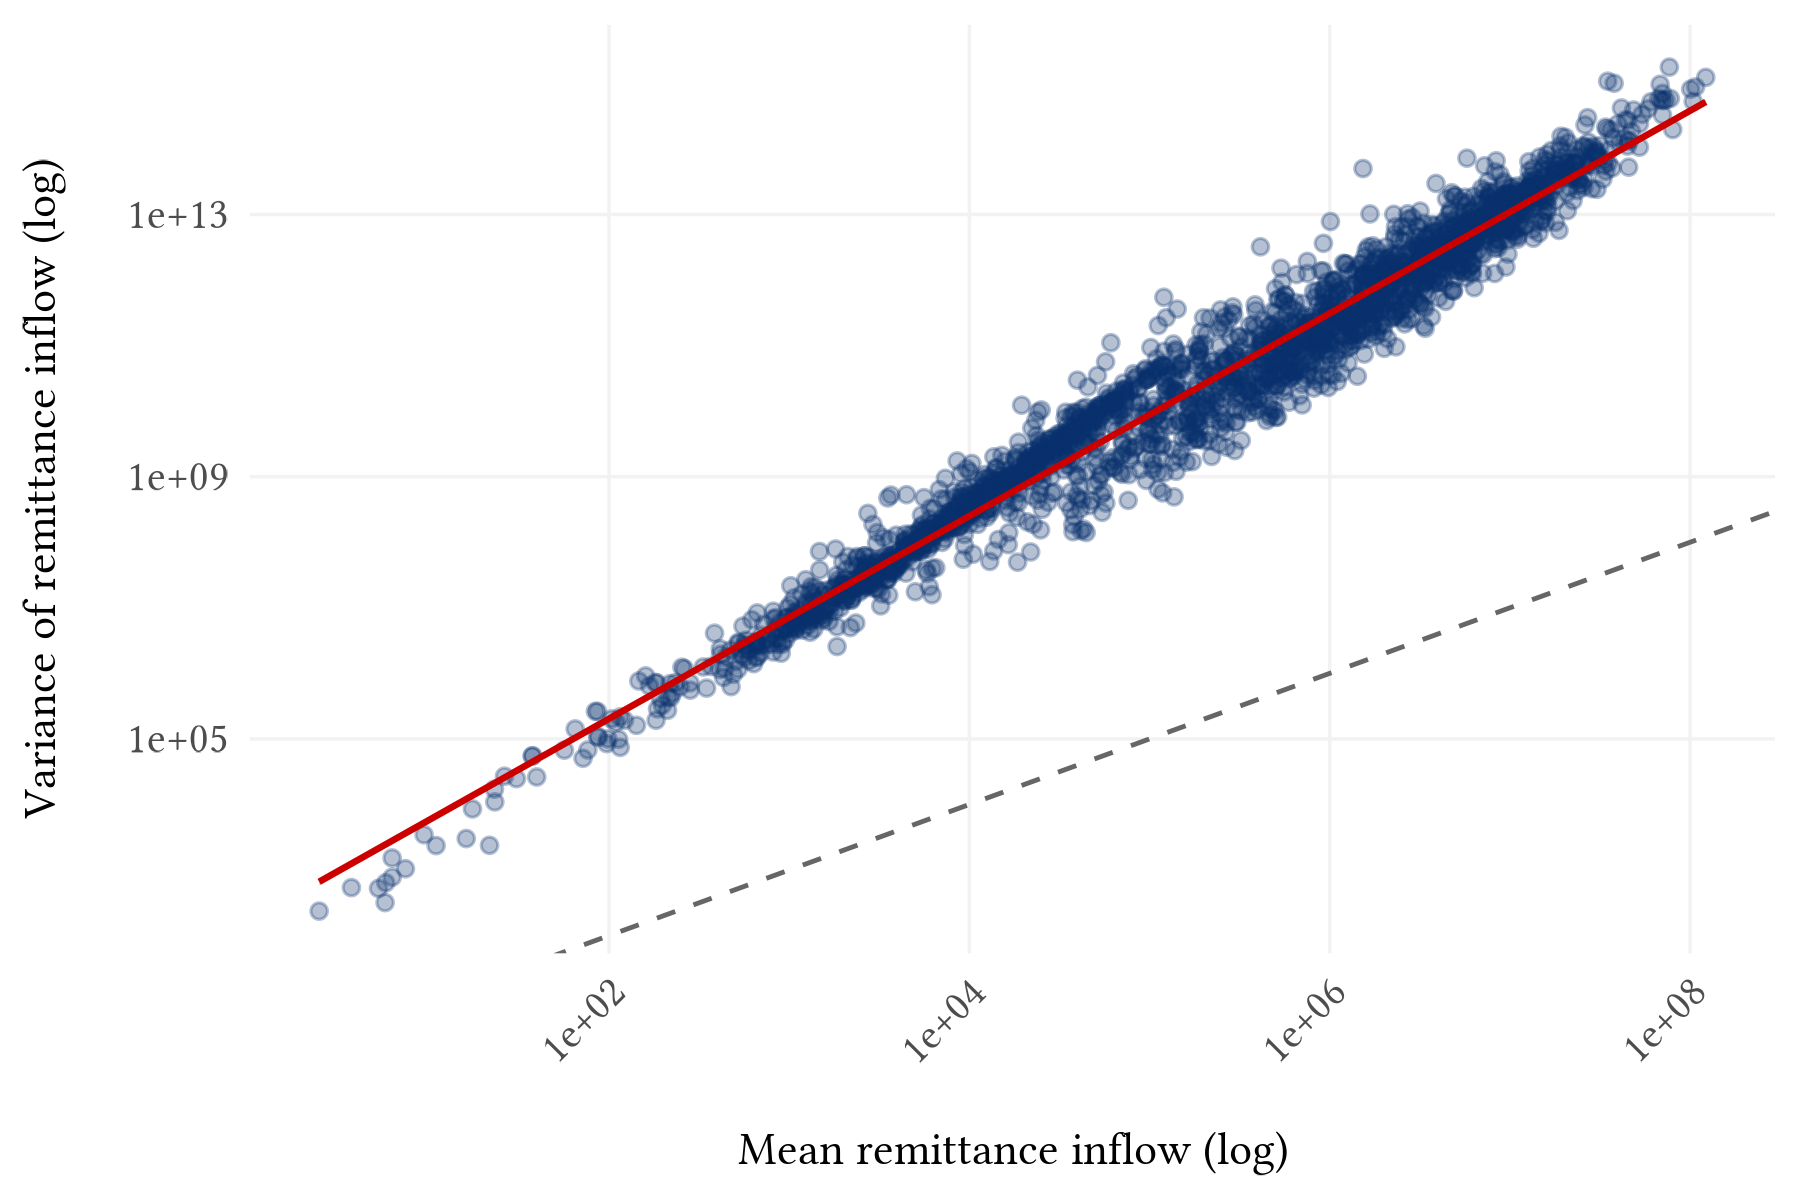
\includegraphics[width=0.8\textwidth]{../figures-tables/ppml/muni-inflows-mean-var.png}
    \caption{Mean-variance relationship of municipality remittance inflows. Each
    point represents a Mexican municipality; axes show the variance against the mean of
    its quarterly inflows over the pre-shock window. The solid
    line is the fitted relationship; the dashed line marks the Poisson
    equidispersion benchmark, where variance equals the mean.}
    \label{fig:mean-variance}
\end{figure}

\section{Results}

Figure \ref{fig:ppml-event-study-fig} shows the result of the PPML event-study estimation, where the vertical dashed line represents the timing of the shock (Q4 2022). The pre-shock coefficients ($\beta_k$ for $k < 0$) are close to zero and statistically insignificant, visually consistent with the parallel trends assumption underlying our DiD design. The point estimate in the quarter of the shock (Q4 2022) is negative and statistically significant at the 1\% level, indicating that municipalities with higher exposure to Florida experienced a larger drop in remittance inflows immediately following the shock. Specifically, a one percentage point increase in Florida exposure is associated with a 0.16\% decrease in remittance inflows in the quarter of the shock. In the subsequent quarters, the coefficients become slightly positive but statistically insignificant at the 5\% level, suggesting that the initial negative impact of the shock on remittance inflows dissipated over time. These results suggest that the Hurricane Ian shock had a significant, but short lived impact on remittance flows, suggesting a rapid re-adjustment of remittance networks after the shock (connection to the model?). However, the fact that the point estimates in the post-shock period are positive, altough not statistically significant, may be indicate a potential overshooting of remittance inflows due to post-shock reconstruction period, or some form of spillover effects through migrant networks in other states, which we will investigate in the next chapter.
\begin{figure}[H]
    \centering
    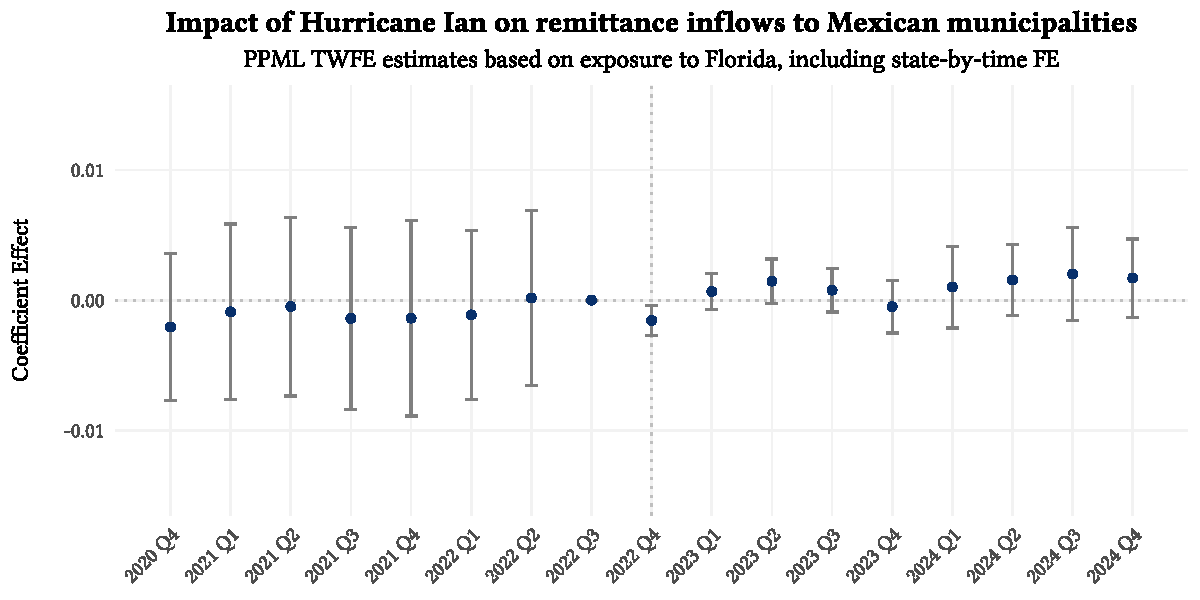
\includegraphics[width=1\textwidth]{../figures-tables/municipality-inflows/muni_did_ppml.pdf}
    \caption{PPML Event Study Estimates}
    \label{fig:ppml-event-study-fig}
\end{figure}
\par
As a robustness check, we also estimate the same event-study specification using spatially clustered errors, following the methodology of \textcite{conley1999}, to account for potential spatial correlation in remittance inflow shocks affecting neighboring municipalities. The results, shown in Figure \ref{fig:ppml-event-study-conley}, are qualitatively similar to the baseline specification, with the main difference being the thighter confidence intervals in the preperiod as buffer distance increases, and slightly wider in the post-shock period. Given that the results are robust to both clustering methods, and that the spatial clustering specification doesn't produce positive definite variance-covariance matrices for buffer distances above 50km, we consider the municipality-level clustering as our baseline specification.
\begin{figure}[H]
    \centering
    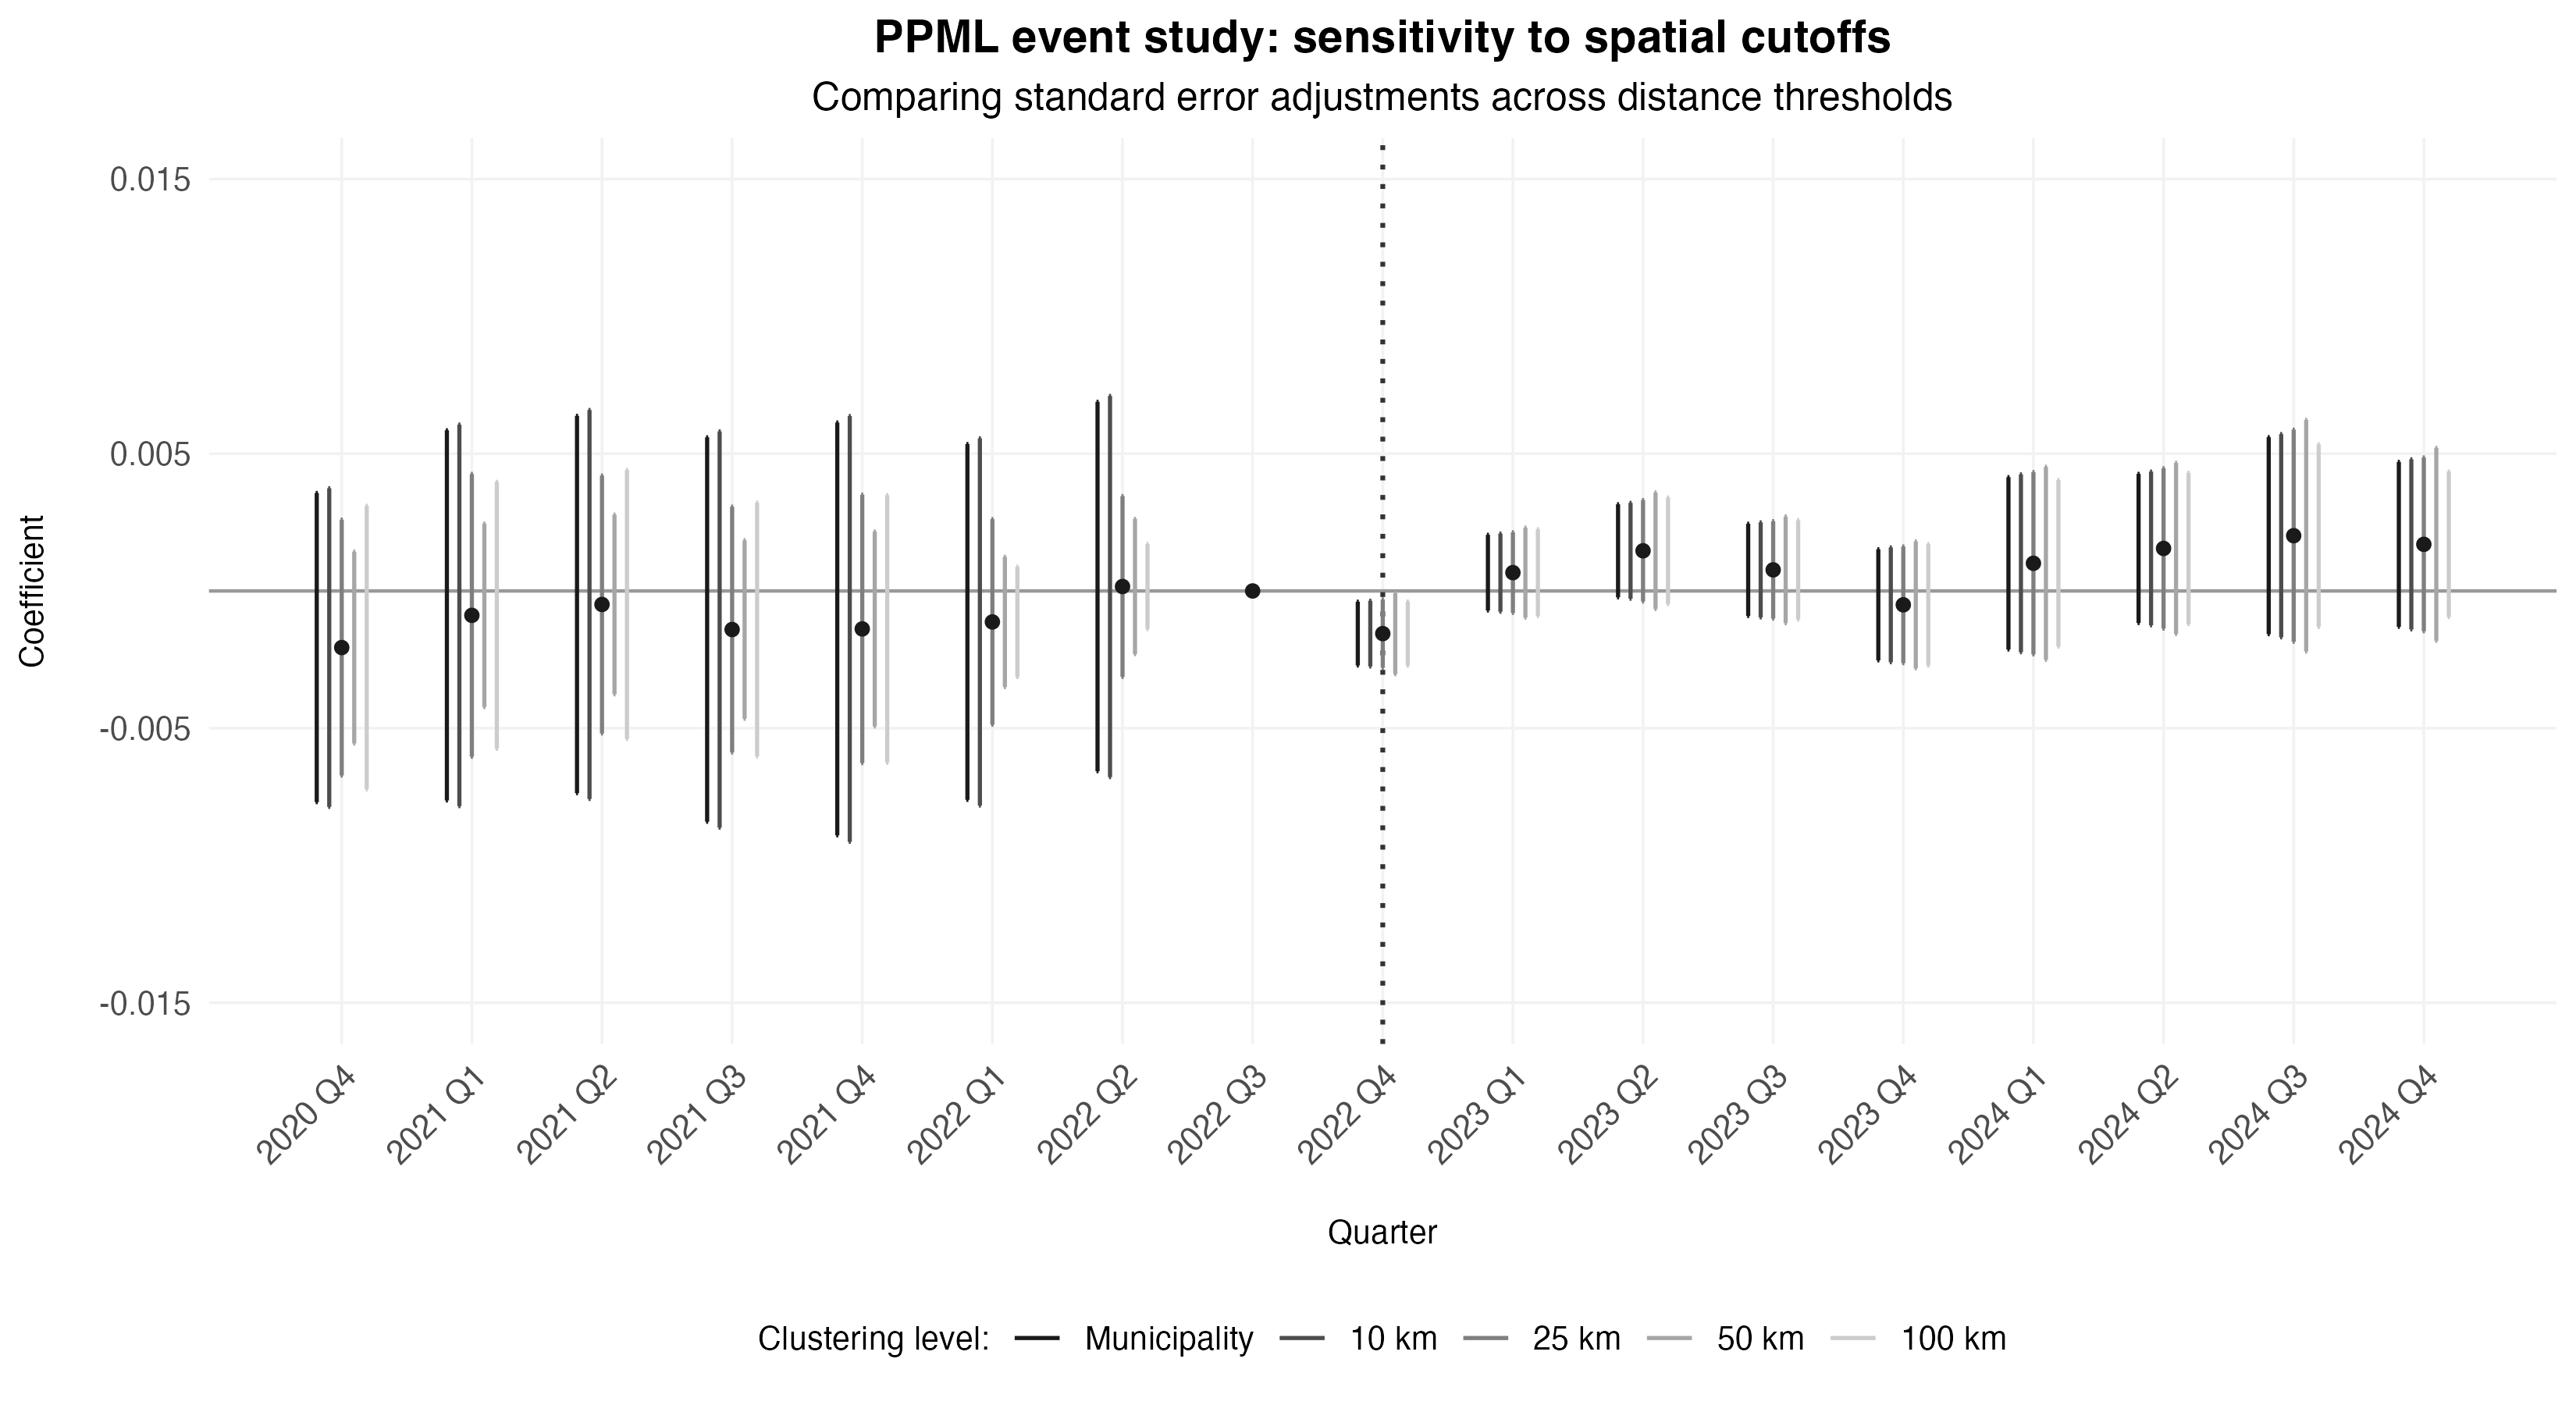
\includegraphics[width=1\textwidth]{../figures-tables/municipality-inflows/muni_spatial_clustering.png}
    \caption{PPML Event Study Estimates with Conley Standard Errors for Different Buffer Distances}
    \label{fig:ppml-event-study-conley}
\end{figure}

\section{Is the Response Specific to Florida?}
\label{sec:identification}

Conditioning on California and Texas exposure leaves the Florida impact coefficient essentially unchanged at $-0.0013$ ($p = 0.034$), while the California and Texas impact coefficients are themselves flat and insignificant ($+0.0004$ and $-0.0001$, respectively). The contraction at landfall is thus specific to Florida exposure and is not correlated with migration to other major destinations.

This rules out a common migration trend as the driver, but it tests only whether exposure to other destinations moves independently at the shock. It leaves open a separate question: whether the Florida response itself depends on a municipality's ties to those destinations. If migrants in Texas or California adjust their own transfers when the municipalities they send to are hit by the Florida shock, the Florida coefficient would already net out that within-network adjustment rather than measure the direct contraction alone. We take up this possibility in the next chapter, where the additive exposures of this section enter interactively to ask how the Florida effect varies across the migrant network.

\footnote{We assess robustness to violations of parallel trends using the relative-magnitudes approach of \textcite{rambachan_roth_2023}, reporting the breakdown value $\bar{M}$ (the largest pre-to-post violation ratio for which the effect stays significant; $\bar{M}=1$ is a conventional lower bound). The baseline Florida-only effect breaks down at $\bar{M}=0.15$ and the netted specification of Section~\ref{sec:identification} at $\bar{M}=0.04$. The sign and timing of the response are thus credible, but its magnitude is fragile, as expected given the dispersed, complex network of remittance flows, which motivates the spillover analysis that follows.}